\graphicspath{ {Figures/interoperability/} }
\chapter{Διασυνδεσιμότητα}\label{ch:Interoperability}
\section{Απαιτήσεις}

\section{Πρωτόκολλα επικοινωνίας}

Το HL7 αναφέρεται στο επίπεδο υγείας 7 (Health Level 7), μια πλήρως εθελοντική, μη κερδοσκοπική οργάνωση υγείας που ενεπλάκη στην ανάπτυξη διεθνών προτύπων υγειονομικής περίθαλψης. Ο όρος HL7 αναφέρεται επίσης σε μερικά από τα συγκεκριμένα πρότυπα που δημιουργούνται από τον οργανισμό, όπως για παράδειγμα: HL7 v2.x, v3.0 κ.α.
Το HL7 και τα μέλη του αφιερώνονται στην παροχή ενός περιεκτικού πλαισίου (και των σχετικών προτύπων) για την ανταλλαγή, την ολοκλήρωση, τη διανομή και την ανάκτηση των ηλεκτρονικών πληροφοριών υγείας. Τα πρότυπα, που υποστηρίζουν την κλινική πρακτική και τη διαχείριση, παράδοση και αξιολόγηση των υγειονομικών υπηρεσιών, είναι τα περισσότερο χρησιμοποιούμενα παγκοσμίως.
Ηλεκτρονικός φάκελος ασθενών με χρήση XML Services και BPEL 69 Web

Τμήμα Ψηφιακών Συστημάτων - Πανεπιστήμιο Πειραιώς
Τα νοσοκομεία συνήθως χρησιμοποιούν πολλά διαφορετικά ηλεκτρονικά υπολογιστικά συστήματα για όλες τις λειτουργίες τους, από την τιμολόγηση των αρχείων μέχρι την παρακολούθηση ασθενούς. Όλα αυτά τα συστήματα πρέπει να επικοινωνήσουν το ένα με το άλλο (διεπαφή) όταν λαμβάνουν τις νέες πληροφορίες. Το HL7 είναι μια γλώσσα με την οποία τα διάφορα συστήματα υγειονομικής περίθαλψης μπορούν να το κάνουν αυτό. Υπάρχει μια μεγάλη ποσότητα πληροφοριών που τα συστήματα υγειονομικής περίθαλψης πρέπει να μεταβιβάσουν. Η σύνδεση των διάφορων συστημάτων υγειονομικής περίθαλψης είναι δύσκολη χωρίς μια κοινή γλώσσα (όπως το HL7).
Στόχος του HL7 είναι η κλινική διαλειτουργικότητα, δηλαδή «Να παρέχει πρότυπα στις ανταλλαγές, την διαχείριση και την ολοκλήρωση των δεδομένων που υποστηρίζουν την φροντίδα του ασθενούς, αλλά και την διαχείριση, διανομή και αποτίμηση σε ολόκληρο το περιβάλλον της φροντίδας υγείας». Η στρατηγική του HL7 είναι η συνεχής καινοτομία.
Υπόβαθρο και οργανωτική δομή
Ο οργανισμός HL7 έχει αυξηθεί από 14 μέλη το 1987 σε πάνω από 2200 μέλη παγκοσμίως σήμερα, συμπεριλαμβανομένων 500 εταιρικών μελών και διεθνείς θυγατρικές σε 33 χώρες. Αυτά τα μέλη μοιράζονται μια δέσμευση, για την ανάπτυξη και την πρόοδο των κλινικών και διοικητικών προτύπων στην υγειονομική περίθαλψη. Χρησιμοποιώντας ένα καθορισμένο με σαφήνεια σύνολο λειτουργικών διαδικασιών, τα μέλη του HL7 - συμπεριλαμβανομένων των προμηθευτών, των συμβούλων και των πληρωτών - έχουν πείρα τεχνολογίας πληροφοριών σε όλα τα τμήματα της βιομηχανίας υγειονομικής περίθαλψης. Συλλογικά, αναπτύσσουν τα πρότυπα με σκοπό να αυξήσουν την αποτελεσματικότητα, την αποδοτικότητα και την ποιότητα παράδοσης υγειονομικής περίθαλψης.
Ο οργανισμός διευθύνεται από ένα διοικητικό συμβούλιο, το οποίο περιλαμβάνει οκτώ εκλεγμένες θέσεις και τρεις διορισμένες θέσεις. Τα μέλη του HL7 είναι συλλογικά γνωστά ως «ομάδα εργασίας». Η ομάδα εργασίας είναι αρμόδια για τον καθορισμό του HL7 τυποποιημένου πρωτοκόλλου και αποτελείται από τις μόνιμες διοικητικές επιτροπές, τις ομάδες ειδικού ενδιαφέροντος και τις τεχνικές επιτροπές. Οι μόνιμες διοικητικές επιτροπές εστιάζουν στις οργανωτικές ή προωθητικές δραστηριότητες, όπως η εκπαίδευση, η εφαρμογή, η διαφήμιση, η έκδοση και βελτίωση απόδοσης και η σχεδίαση. Οι ομάδες ειδικού ενδιαφέροντος χρησιμεύουν ως ένα πεδίο δοκιμής για να ερευνήσουν τις νέες περιοχές που μπορεί να χρειαστούν κάλυψη στα HL7 δημοσιοποιημένα πρότυπα. Οι Τεχνικές
Ηλεκτρονικός φάκελος ασθενών με χρήση XML Services και BPEL 70 Web

Τμήμα Ψηφιακών Συστημάτων - Πανεπιστήμιο Πειραιώς
Επιτροπές είναι άμεσα αρμόδιες για το περιεχόμενο των προτύπων, πλαισιώνοντας την πραγματική γλώσσα των προδιαγραφών.
Μια συχνή παρερμηνεία για το HL7 είναι ότι η ομάδα αναπτύσσει λογισμικό. Στην πραγματικότητα, η αρχική αποστολή του HL7 είναι να δημιουργηθούν ευέλικτα, χαμηλού κόστους πρότυπα, οδηγίες και μεθοδολογίες που θα επιτρέψουν την ανταλλαγή και τη διαλειτουργικότητα των ηλεκτρονικών χαρτών υγείας. Τέτοιες οδηγίες ή πρότυπα δεδομένων είναι ένα σύνολο κανόνων που επιτρέπουν στις πληροφορίες να μοιραστούν και να υποβληθούν σε επεξεργασία κατά τρόπο ομοιόμορφο και συνεπή. Χωρίς πρότυπα δεδομένων, οι οργανώσεις υγειονομικής περίθαλψης δεν θα μπορούσαν να μοιραστούν εύκολα κλινικές πληροφορίες. Θεωρητικά, αυτή η δυνατότητα να ανταλλαχθούν οι πληροφορίες πρέπει να βοηθήσει να ελαχιστοποιηθεί η τάση να είναι η ιατρική φροντίδα γεωγραφικά απομονωμένη και ιδιαίτερα μεταβλητή.
Οι περισσότεροι οργανισμοί ανάπτυξης προτύπων (Standards Ανάπτυξη Οργανισμοί), συμπεριλαμβανομένου του HL7, αναπτύσσουν πρότυπα για μια ιδιαίτερη περιοχή υγειονομικής περίθαλψης όπως το φαρμακείο, οι ιατρικές συσκευές, οι συναλλαγές απεικόνισης ή ασφάλειας. Το φάσμα του HL7 είναι κλινικά δεδομένα και δεδομένα διαχείρισης. Τα πρότυπα ανταλλαγής μηνυμάτων είναι ιδιαίτερα σημαντικά επειδή καθορίζουν πως οι πληροφορίες συσκευάζονται και διαβιβάζονται από το ένα συμβαλλόμενο μέρος σε άλλο. Τέτοια πρότυπα θέτουν τη γλώσσα, τύπους δομών και δεδομένων που απαιτούνται για τη συνεχή ολοκλήρωση από ένα σύστημα σε άλλο. Αυτή την περίοδο, τα πρότυπα ανταλλαγής μηνυμάτων του HL7 υποστηρίζονται από κάθε σημαντικό προμηθευτή πληροφοριακών συστημάτων στις Ηνωμένες Πολιτείες.
Τομείς ενδιαφέροντος
Το 1994, το HL7 αναγνωρίστηκε από το ANSI (διεθνή οργανισμό προτύπων). Στα έτη από την ίδρυσή του, το HL7 έχει επεκτείνει την επιρροή του πέρα ​​από τα παραδοσιακά πρωτόκολλα ανταλλαγής μηνυμάτων. Σήμερα οι πρωτοβουλίες ανάπτυξης προτύπων HL7 περιλαμβάνουν τα εξής:
- Τυποποίηση της απεικόνισης γνώσης
- Προδιαγραφή των συστατικών για τη διαχείριση πλαισίου
- Υποστήριξη για την ανταλλαγή στοιχείων υγειονομικής περίθαλψης χρησιμοποιώντας
μεσίτες αιτήματος αντικειμένου (object αιτήματος μεσίτη)
Ηλεκτρονικός φάκελος ασθενών με χρήση XML Services και BPEL 71 Web

Τμήμα Ψηφιακών Συστημάτων - Πανεπιστήμιο Πειραιώς
- Τυποποίηση των δομών εγγράφων XML
- Λειτουργικές προδιαγραφές για ένα ηλεκτρονικό αρχείο υγείας
- Δουλειά στον τομέα της ασφάλειας, της μυστικότητας, της εμπιστευτικότητας και της
υπευθυνότητας
Τέτοια καινοτομία έχει επιτρέψει τα πάντα, από τη διαθεσιμότητα ενός διαδικτυακού ιατρικού αρχείου ασθενούς στη συνταγή ενός φαρμακείου που ανταλλάσσεται με ένα έγγραφο XML HL7. Στην πραγματικότητα, η HL7 αρχιτεκτονική φακέλου ασθενούς στην έκδοση 3.0 επιτρέπει ένα κοινό σχήμα για την ανταλλαγή του ιατρικού αρχείου ενός ασθενή μεταξύ των διαφορετικών συστημάτων νοσοκομείων ή ακόμα και των διαφορετικών νοσοκομείων. Αυτό το HL7 πρότυπο χρησιμεύει ως θεμέλιο για το ηλεκτρονικό ιατρικό αρχείο.
Ο σκοπός των δραστηριοτήτων του HL7 δεν περιορίζεται στο ηλεκτρονικό ιατρικό αρχείο, εντούτοις. Πράγματι, οι πρόσφατες δραστηριότητες και τα πρότυπα HL7 έχουν περιλάβει τη διαμόρφωση και τη μεθοδολογία, το λεξιλόγιο, την υποστήριξη κλινικής απόφασης, την οικονομική διαχείριση, τη διοίκηση, τη ρυθμισμένη κλινική έρευνα και τη διαχείριση πληροφοριών, το σχεδιασμό και τις διοικητικές μέριμνες, τις κλινικές οδηγίες, τα κυβερνητικά προγράμματα, το φάρμακο, την ασφάλεια και την υπευθυνότητα, τα πρότυπα XML, και την απάντηση δημόσιας υγείας και έκτακτης ανάγκης.
Το HL7 έχει επιτρέψει τη διαλειτουργικότητα μεταξύ των συστημάτων ηλεκτρονικής διοίκησης ασθενών (Patient Συστημάτων Διαχείρισης), των συστημάτων ηλεκτρονικής πρακτικής διαχείρισης (Ηλεκτρονική Διαχείριση Πρακτικής), των συστημάτων εργαστηριακών πληροφοριών (Εργαστήριο Πληροφοριακών Συστημάτων). Το HL7 καλύπτει τον πλήρη κύκλο ζωής μιας προδιαγραφής προτύπων συμπεριλαμβανομένης της ανάπτυξης, της υιοθέτησης, της αναγνώρισης αγοράς και της χρησιμοποίησης.
Συγκεκριμένοι στόχοι HL7
Ο κύριος στόχος του HL7 είναι η ανάπτυξη ενός προτύπου το οποίο θα επιτρέπει τη μεταφορά και ανταλλαγή δεδομένων (ιατρικής πληροφορίας) μεταξύ εντελώς διαφορετικών οργανισμών και συστημάτων. Αναλυτικότερα:
Ηλεκτρονικός φάκελος ασθενών με χρήση XML Services και BPEL 72 Web

Τμήμα Ψηφιακών Συστημάτων - Πανεπιστήμιο Πειραιώς
- Ανάπτυξη κατανοητών, με δυνατότητα επέκτασης προτύπων που επιτρέπουν δομημένη, κωδικοποιημένη πληροφορία υγειονομικής περίθαλψης, που ανταλλάσσεται μεταξύ πληροφοριακών εφαρμογών διατηρώντας τη σημασία.
- Ανάπτυξη μιας επίσημης μεθοδολογίας για την υποστήριξη της δημιουργίας προτύπων HL7.
- Εκπαίδευση της βιομηχανίας υγειονομικής περίθαλψης, τους φορείς χάραξης πολιτικής, και το ευρύ κοινό σχετικά με τα οφέλη της τυποποίησης πληροφοριών υγειονομικής
περίθαλψης γενικά και για τα HL7 πρότυπα συγκεκριμένα.
- Προώθηση της χρήσης του HL7 προτύπων παγκοσμίως μέσω της δημιουργίας διεθνών
HL7 θυγατρικών οργανισμών, οι οποίοι συμμετέχουν στην ανάπτυξη των προτύπων HL7.
- Συνεργασία με άλλες οργανώσεις ανάπτυξης προτύπων και εθνικούς και διεθνείς οργανισμούς (π.χ. ANSI και ISO), στις περιοχές υποδομής υγειονομικής περίθαλψης και
πληροφοριών για προώθηση της χρήσης των υποστηρικτικών και συμβατών προτύπων.
- Συνεργασία με τους χρήστες τεχνολογίας πληροφοριών υγειονομικής περίθαλψης για να εξασφαλιστεί πως τα HL7 πρότυπα καλύπτουν τις πραγματικές απαιτήσεις, και ότι οι προσπάθειες ανάπτυξης κατάλληλων προτύπων δημιουργούνται από τον οργανισμό HL7
για να καλύψουν τις προκύπτουσες απαιτήσεις.
Η RIM - ISO / HL7 21731
Το μοντέλο αναφοράς πληροφορίας (RIM) είναι ο ακρογωνιαίος λίθος της ανάπτυξης της έκδοσης 3 του HL7 και ένα αναγκαίο μέρος της μεθοδολογίας ανάπτυξης του HL7. Το RIM εκφράζει τα δεδομένα που απαιτούνται σε μια συγκεκριμένη έκφανση της κλινικής λειτουργίας και παρέχει μια συγκεκριμένη αναπαράσταση των μεταπληροφοριών (σημασιολογία) και λεξικών συνδέσεων που υπάρχουν μεταξύ των μηνυμάτων που μεταφέρονται στο επίπεδο του HL7.
Επίπεδο ανάπτυξης (πλαίσιο ανάπτυξης) HL7 - ISO / HL7 27931
Το επίπεδο ανάπτυξης (HDF) του HL7 προτύπου 3 είναι μια διαδικασία συνεχούς εξέλιξης που αποζητά να αναπτύξει πρότυπα και ορισμούς που αναπτύσσουν τη διαλειτουργικότητα μεταξύ πληροφοριακών συστημάτων υγείας.
Το HDF επίσης καταγράφει τις διαδικασίες, εργαλεία, κανόνες και οτιδήποτε σχετίζεται με τα πρότυπα ανάπτυξης του HL7. Κάποια στιγμή, το HL7 θα περιλαμβάνει όλες τις προδιαγραφές των προτύπων του
Ηλεκτρονικός φάκελος ασθενών με χρήση XML Services και BPEL 73 Web

Τμήμα Ψηφιακών Συστημάτων - Πανεπιστήμιο Πειραιώς
HL7, συμπεριλαμβανομένων των καινούριων προτύπων που θα προκύψουν από την ανάλυση πληροφοριακών συστημάτων υγείας.
Ανταλλαγή μηνυμάτων στο HL7 v3
Στην έκδοση 3, το πρότυπο ανταλλαγής μηνυμάτων προσδιορίζει μια σειρά από ηλεκτρονικά μηνύματα για να υποστηριχθούν όλες οι ιατρικές ροές εργασίας. Τα μηνύματα αυτά βασίζονται στη σύνταξη της XML.
4.4.2 Συνοχή φακέλου φροντίδας (Συνέχεια της Φροντίδας Record, CCR)
Η συνοχή φακέλου φροντίδας (CCR) είναι ένα πρότυπο φακέλου υγείας που αναπτύσσεται από κοινού από την ASTM International, τον Ιατρικό Σύλλογο Μασαχουσέτης (Massachusets Ιατρικό Σύλλογο, MMS), ΤΟ Χιμς, την αμερικανική ακαδημία των οικογενειακών παθολόγων (Αμερικανική Ακαδημία Οικογενειακών Ιατρών, AAFP ), την αμερικανική ακαδημία παιδιατρικής (American Academy of Pediatrics, AAP), και από άλλους προμηθευτές πληροφορικής υγείας.
Το πρότυπο CCR είναι πρότυπο περίληψης υγείας ασθενούς. Είναι ένας τρόπος να δημιουργηθούν ευέλικτα έγγραφα που περιέχουν τις πιο σχετικές και έγκαιρες / έγκυρες πληροφορίες υγείας για έναν ασθενή, και να σταλούν αυτές ηλεκτρονικά από έναν γιατρό σε άλλον. Περιέχει διάφορα τμήματα, όπως οι ασφαλιστικές πληροφορίες του ασθενούς, η διάγνωση και ο κατάλογος προβλημάτων, τα φάρμακα, οι αλλεργίες και το σχέδιο περίθαλψης. Όλα αυτά αντιπροσωπεύουν ένα στιγμιότυπο "στιγμιότυπο" των στοιχείων υγείας ενός ασθενούς που μπορεί να είναι χρήσιμα ή και ακόμη να σώσουν ζωές. Το ASTM CCR πρότυπο έχει σχεδιαστεί για να επιτρέψει την εύκολη χρήση από έναν παθολόγο χρησιμοποιώντας ένα ηλεκτρονικό σύστημα αρχείων υγείας.
Επειδή εκφράζεται με την τυποποιημένη γλώσσα ανταλλαγής δεδομένων XML, ένα CCR μπορεί αν δημιουργηθεί, να διαβαστεί και να ερμηνευθεί από οποιεσδήποτε εφαρμογές λογισμικού ηλεκτρονικού φακέλου ασθενούς. Ένα CCR μπορεί επίσης να εξαχθεί με άλλη μορφή, όπως PDF και το Microsoft Word.
Το CCR γίνεται το επιλεγμένο πρότυπο για την ανταλλαγή πληροφοριών ασθενών και για την βιομηχανική προσπάθεια να βελτιωθεί η ποιότητα της δυνατότητας μεταφοράς πληροφοριών υγείας για την αντιμετώπιση λαθών. Το CCR φέρει στην επιφάνεια την δυνατότητα

	\subsection{HL7 messaging v2 και v3}

	\subsection{CDA Documents}
	

		
\section{Δυνατότητες διασύνδεσης με άλλα υποσυστήματα}

	\subsection{Ηλεκτρονική Συνταγογράφηση}
	
		Η διαδικασία της συνταγογράφησης φαρμάκων μπορεί να είναι ιδιαίτερα περίπλοκη και επιρρεπής σε λάθη, με
δυσμενείς επιπτώσεις για την ασφάλεια των ασθενών. Η πρόληψη των επιπλοκών που μπορούν να προκύψουν λόγω ακατάλληλης συνταγογράφησης είναι μία πρόκληση που αντιμετωπίζει το σύστημα υγείας σε παγκόσμιο επίπεδο. Οι λανθασμένες φαρμακευτικές αγωγές, οι παρενέργειες των φαρμάκων και η αποτυχία σωστής συνταγογράφησης που να συντελέσει στην θεραπεία του ασθενούς εκτός του γεγονότος ότι αποτελεί απειλή για την ασφάλεια του, οδηγεί σε σημαντικές δαπάνες για τα συστήματα υγειονομική περίθαλψης. Οι πληροφορίες σχετικά με το ιστορικό του ασθενούς, τις αλλεργίες, τις παρελθοντικές και τις τρέχουσες φαρμακευτικές αγωγές καθώς και τα εργαστηριακά αποτελέσματα του είναι άκρως απαραίτητα ώστε οι κλινικοί ιατροί να συνταγογραφήσουν την κατάλληλη φαρμακευτική αγωγή, αλλά είναι συχνά δεν είναι διαθέσιμα. \cite{prescribingErrors} Στην Ελλάδα ειδικότερα, υφίσταται το πρόβλημα της αλόγιστης ή πλασματικής συνταγογράφησης με αποτέλεσμα να  χρειάζονται μέτρα για την επαναφορά της αξιοπιστίας της διαδικασίας.  Χαρακτηριστικό παράδειγμα είναι τα στοιχεία του Υπουργείου Υγείας και Κοινωνικής Ασφάλισης, με βάση τα οποία το έτος 2009 εκτελεστήκαν στην Ελλάδα περίπου 100 εκατομμύρια ετησίως ενώ αντίστοιχα στην Δανία εκτελέστηκαν μόνο 15 εκατομμύρια συνταγές.


		Με τον όρο ηλεκτρονική συνταγογράφηση (e-prescription) σύμφωνα με το Εθνικό Σύστημα Υγείας στην Αγγλία αναφερόμαστε στην αξιοποίηση των ηλεκτρονικών συστημάτων για την διευκόλυνση και την ενίσχυσης της επικοινωνίας μίας ιατρικής εντολής ή συνταγής, βοηθώντας στην επιλογή, τη διαχείριση και την προμήθεια ενός φαρμάκου μέσω της γνώσης και υποστήριξης αποφάσεων, παρέχοντας μια διαδρομή ελέγχου για το σύνολο της διαδικασίας χρήσης των φαρμάκων.  Τα συστήματα ηλεκτρονικής συνταγογράφησης που προσφέρουν ηλεκτρονική υποστήριξη στους κλινικούς ιατρούς έχουν σχεδιαστεί για να βοηθήσουν στην περίπλοκη διαδικασία της συνταγογράφησης. \cite{Kierkegaard2013} Επιτρέπουν σε έναν γιατρό, έναν φαρμακοποιό, μία νοσηλεύτρια να διαβιβάσει χωρίς σφάλματα, ακριβείς και κατανοητές συνταγές ηλεκτρονικά, μέσα από τον φορέα παροχής υπηρεσιών υγείας, στο φαρμακείο.  \cite{eprescr}
		
		
		Τα συστήματα ηλεκτρονικής συνταγογράφησης μπορεί να έχουν λειτουργικές δυνατότητες για την παροχή βασικής υποστήριξης αποφάσεων, όπως ο έλεγχος για τυχόν αλλεργίες στα φάρμακα, βασικές κατευθυντήριες γραμμές για τη δοσολογία, τεστ για πιθανές αντιδράσεις μεταξύ φαρμάκων κ.λ.π. Τα συστήματα αυτά είναι ιδιαίτερα χρήσιμα στο τεχνικό κομμάτι της συνταγογράφησης κατάλληλων φαρμάκων, καθώς προσφέρουν λειτουργίες όπως ο υπολογισμός της σωστής δόσης ή ο εντοπισμός αλληλεπιδράσεων μεταξύ των φαρμάκων. \cite{Kart2008}

		Τα συστήματα ηλεκτρονικής συνταγογράφησης χωρίζονται σε δύο κατηγορίες:
		
		\begin{itemize}
		
		\item Τα αυτόνομα συστήματα (stand alone systems). Πρόκειται για λειτουργικά συστήματα τα οποία είναι εγκατεστημένα στους ηλεκτρονικούς υπολογιστές  και χρησιμοποιούνται είτε αυτόνομα είτε μέσω σύνδεσης στο διαδίκτυο.  Τα συστήματα αυτά χρησιμοποιούνται κυρίως για τον έλεγχο θεμάτων ασφάλειας και γίνεται προσπάθεια αντικατάστασης τους από τα ολοκληρωμένα συστήματα συνταγογράφησης.

		\item Τα ολοκληρωμένα συστήματα συνταγογράφησης (Electronic Health Record, EHR Systems). Στα συστήματα αυτά ο ιατρός έχει στην διάθεση του όλο το ιστορικό του ασθενούς, τα αποτελέσματα των εξετάσεων του και τα χρησιμοποιεί για να βοηθηθεί στην επιλογή της κατάλληλης δραστικής ουσίας. Οι συναγερμοί ασφαλείας στην περίπτωση αυτή είναι πιο εξειδικευμένοι και ακριβείς.  

		\end{itemize}
		

		Συνοπτικά τα συστατικά της ηλεκτρονικής συνταγογράφησης μπορούν να κατηγοριοποιηθούν σε βασικές δυνατότητες συνταγογράφησης, πληροφορίες για το πλάνο υγείας και τις κλινικές ειδοποιήσεις (clinical alerts).  Οι δυνατότητες συνταγογράφησης περιλαμβάνουν μια λίστα φαρμάκων, οδηγίες για τους ασθενείς, τον αριθμός των εγκεκριμένων ποσοτήτων, σχόλια του γιατρού που συνταγογραφεί προς τον φαρμακοποιό, καθώς και το πεδίο PRN. Οι πληροφορίες για το πλάνο υγείας του ασθενούς περιλαμβάνουν την ιατρική ασφάλεια που έχει και το ιστορικό των φαρμακευτικών αγωγών. Τέλος, οι κλινικές ειδοποιήσεις  βασίζονται στα δημογραφικά στοιχεία και στα στοιχεία του ιατρικού ιστορικού του ασθενούς και περιλαμβάνουν τις αντιδράσεις μεταξύ των φαρμάκων, τις αλλεργίες, τις προειδοποιήσεις για συγκεκριμένες ηλικιακές ομάδες και την κατάλληλη προσαρμογή της δόσης με βάση το βάρος του ασθενούς. \cite{prescribing} 
		
		
		Τα βασικά συστατικά ενός συστήματος ηλεκτρονικής συνταγογράφησης είναι \cite{Grossman2012}:

		\begin{itemize}

		\item Ο παραπέμπων ιατρός. Ο θεράπων ιατρός είναι ο κύριος χρήστης  του συστήματος. Για την σύνδεση του στο σύστημα ακολουθείται μιας διαδικασία επαλήθευσης ώστε να επιβεβαιωθεί η ταυτότητά του. 
Οι αναζητήσεις του θεράποντα ιατρού στην βάσης δεδομένων που περιέχει τους φακέλους των ασθενών πραγματοποιείται με τη χρήση ειδικών πληροφοριών για τον ασθενή, συνήθως το ΑΜΚΑ για Ελλάδα ή τον αριθμό κοινωνικής ασφάλισης (social security number) στον εξωτερικό. Μόλις προσπελαστεί το σωστό αρχείο του ασθενούς, ο ιατρός εξετάζει τις ιατρικές πληροφορίες που περιέχει και προσθέτει ή ενημερώνει μία συνταγή στον ιατρικό φάκελο.
		
		\item Ο κόμβος συναλλαγών. Αποτελεί τον κοινό σύνδεσμο μεταξύ όλων των φορέων (παραπέμπων ιατρός και φαρμακείο). Αποθηκεύει και διατηρεί ένα κύριο κατάλογο των ασθενών για να υπάρχει η δυνατότητα γρήγορης πρόσβασης στις ιατρικές πληροφορίες των ασθενών, καθώς και στην λίστα των φαρμακείων. Όταν ο παραπέμπων ιατρός ανεβάσει κάποια νέα συνταγή στον φάκελο του ασθενούς, τότε αυτή μεταφέρεται αυτόματα και στον κόμβο συναλλαγών. Ο κόμβος συναλλαγών θα στείλει αυτόματα τις πληροφορίες  με στο κεντρικό σύστημα διαχείρισης το οποίο θα απαντήσει με πληροφορίες σχετικά με την καταλληλότητα του ασθενή και το ιστορικό των φαρμακευτικών αγωγών του.  Ο κόμβος συναλλαγών έπειτα στέλνει τις πληροφορίες στον ιατρό έτσι ώστε να έχει τις απαραίτητες πληροφορίες που του χρειάζονται και να ολοκληρώσει και να εγκρίνει την συνταγή. 
		
		\item Το κεντρικό σύστημα διαχείρισης δεδομένων, στο οποίο βρίσκονται όλα τα στοιχεία ιατρικού φακέλου που ελέγχει την καταλληλότητα του ασθενή καθώς και της συνταγής. Το κεντρικό σύστημα διαχείρισης δεδομένων επικοινώνει με τον ιατρό και το φαρμακείο.
		
		\item Το φαρμακείο που έχει εγκατεστημένο το λογισμικό της ηλεκτρονικής συνταγογράφησης. Το φαρμακείο ανακτά την συνταγή από  το κεντρικό σύστημα διαχείρισης συναλλαγών μέσω του κόμβου συναλλαγών και έχει επιπλέον την ικανότητα να επικοινωνήσει με τον ιατρό και να τον ενημερώσει ότι η παραγγελία εκτελέστηκε. 
		
		\end{itemize}
		
		
		
		\subsubsection{Ηλεκτρονική Συνταγογράφηση στην Ελλάδα}
		
		Η ηλεκτρονική συνταγογράφηση στην Ελλάδα βασίζεται στις οδηγίες του νόμου 3892/2010 (ΦΕΚ 189 Α) «Ηλεκτρονική καταχώριση και εκτέλεση ιατρικών συνταγών και παραπεμπτικών ιατρικών εξετάσεων». Σε αυτόν το νόμο καταγράφονται τα ζητήματα ηλεκτρονικής συνταγογράφησης και τα ζητήματα των ηλεκτρονικών παραπεμπτικών.
		
		Ο υπεύθυνος φορέας στην Ελλάδα είναι η Γενική Γραμματεία Κοινωνικών Ασφαλίσεων του Υπουργείου Εργασίας, Κοινωνικής Ασφάλισης και Πρόνοιας. Το σύστημα υποστηρίζεται ηλεκτρονικά από την Ηλεκτρονική Διακυβέρνηση Κοινωνικής Ασφάλισης (ΗΔΙΚΑ Α.Ε.). Η ΗΔΙΚΑ αποτελεί μια ανώνυμη, μη κερδοσκοπικού χαρακτήρα του δημοσίου την οποία αποζημιώνουν οι εξυπηρετούμενοι φορείς για τις υπηρεσίες του παρέχει, όπως για παράδειγμα το έργο μισθοδοσίας των φορέων.  \cite{idika}
		
		Με τον όρο ηλεκτρονική συνταγογράφηση αναφερόμαστε στη παραγωγή, στην διακίνηση και στον έλεγχο των ιατρικών συνταγών και των παραπεμπτικών για ιατρικές πράξεις, με τη χρήση τεχνολογίας ηλεκτρονικών υπολογιστών και επικοινωνιών, έτσι ώστε να διασφαλίζεται η ασφάλεια, η εγκυρότητα και η διαφάνεια στις πληροφορίες που διακινούνται. Ουσιαστικά, το σύστημα περιλαμβάνει ένα αριθμό από διαδικασίες που σχετίζονται με τη δημιουργία, την εκτέλεση, τη διαχείριση, τον έλεγχο, την εκκαθάριση και την εξόφληση μιας φαρμακευτικής συνταγής ή ενός παραπεμπτικού για ιατρικές πράξεις. Διέπει όλα τα συστήματα και τις τοποθεσίες που εμπλέκονται όπως τα τακτικά ιατρεία των νοσοκομείων ή τα ιδιωτικά ιατρεία, τα κέντρα υγείας, τις κλινικές, τα διαγνωστικά κέντρα, τα φαρμακεία και τα ασφαλιστικά ταμεία.


		
		Το ολοκληρωμένο σύστημα ηλεκτρονικής συνταγογράφησης στην Ελλάδα εξυπηρετεί τους εξής σκοπούς:
		
		\begin{itemize}

		\item  Βοηθά στον αποτελεσματικό εκσυγχρονισμό του συστήματος της φαρμακευτικής περίθαλψης. Οι χειρόγραφες συνταγές έχουν αντικατασταθεί από τις ηλεκτρονικές και η διαδικασία έχει αυτοματοποιηθεί.
		 
		\item Συντελεί στην ταυτοποίηση και τον έλεγχο των εμπλεκομένων για να διασφαλίσει την ακεραιότητα της διαδικασίας και την ευρεία και επιτυχημένη επιχειρησιακή λειτουργία της ηλεκτρονικής συνταγογράφησης.
		
		\item Βελτιώνει την ασφάλεια και την ποιότητα της φροντίδας του ασθενούς. Με την αύξηση του όγκου των φαρμάκων και της πολυπλοκότητα των ιατρικών αναγκών των ασθενών, εφίσταται αυξημένος κίνδυνος σφαλμάτων και παρενεργειών. Η ηλεκτρονική συνταγογράφηση μπορεί να βελτιώσει την ασφάλεια και την ποιότητα της φροντίδας του ασθενούς και να μειώσει τον αριθμό των λαθών
		
		\item Εισάγει και αξιοποιεί τις λειτουργίες της ηλεκτρονικής συνταγογράφησης στην καθημερινή πρακτική.

		\end{itemize}

	\subsubsection{E-prescription }
	
		Το ελληνικό σύστημα ηλεκτρονικής συνταγογράφησης,  το επονομαζόμενο e-precription, καθιερώθηκε το 2013. Πλέον καλύπτει περισσότερο  από το 95\% του συνόλου των συνταγών που γράφονται . Το e-precription δημιουργήθηκε με σκοπό να παρέχει τις εξής λειτουργίες: την ηλεκτρονική καταχώρηση και διαχείριση των συνταγών, την ενίσχυση της γνώσης μέσω της δυνατότητας άμεσης πρόσβασης στις πληροφορίες των φαρμάκων, την υποστήριξη λήψης αποφάσεων καθώς βοηθά την επιλογή των φαρμάκων με διάφορες ειδοποιήσεις, την υποστήριξη κατά την διοίκηση, την δημιουργία ηλεκτρονικών συνδέσμων μεταξύ των νοσοκομείων και των φαρμακείων, τις βελτιώσεις στις ήδη υπάρχουσες εργασιακές διαδικασίες, και τέλος την ανάπτυξης μιας διαδρομή ελέγχου για το σύνολο της χρήσης των φαρμάκων.  \cite{miller}
		
		Το e-prescription πραγματοποιεί την ηλεκτρονική επεξεργασία των συνταγών για όλους τους ασθενείς, οι οποίοι είναι ασφαλισμένοι σε κάποιον από τους εθνικούς φορείς ασφαλίσεων.Το σύστημα εστιάζει ιδιαιτέρως στην βελτίωση της ασφάλειας των ασθενών, την καλύτερη αξιοποίηση των πόρων και στην διαλειτουργικότητα με άλλα εθνικά ή ευρωπαϊκά συστήματα. Είναι διαθέσιμο μέσω του διαδικτύου (internet) και αποτελεί ένα αυτόνομο ηλεκτρονικό σύστημα εισόδου στο οποίο κάθε υποβολή συνταγής είναι ασφαλής και αναγνωρίζεται από έναν μοναδικό αριθμό. Στο σχήμα \ref{fig:prescr} απεικονίζεται η συνολική δομή του συστήματος. \cite{pangalos}
		
		Ο θεράπων ιατρός δημιουργεί τις συνταγές οι οποίες αποθηκεύονται στην εθνική βάση του συστήματος e-prescription , η οποία βρίσκεται στην ΗΔΙΚΑ. \cite{idika}Όταν ένα φαρμακείο θέλει να εκτελέσει μία συνταγή την  "διαβάζει" από την κεντρική βάση. Οι πληροφορίες ου βρίσκονται στην βάση δεδομένων είναι διαθέσιμες (μέσω ασφαλούς on-line πρόσβασης, ή εξειδικευμένων περιοδικών αναφορών) σε όλα τα σχετικά και ενδιαφερόμενα μέρη (Οργανισμοί Ασφάλισης Υγείας, Υπουργείο Υγείας, εποπτικές αρχές, κλπ). Οι συνταγές που έχουν εκτελεστεί από τα φαρμακεία  ελέγχονται από τους οργανισμούς ασφάλισης, ενώ το σύστημα e-prescription χρησιμοποιείται για να διασταυρώνονται οι έλεγχοι. \cite{papala}

	Η εφαρμογή του e-prescription είναι μία διαδικτυακή εφαρμογή. Στο σύστημα έχουν πρόσβαση μόνο εξουσιοδοτημένοι χρήστες (ιατροί, φαρμακοποιοί, κλπ), οι οποίοι αναγνωρίζονται και αποκτούν άδεια πρόσβασης μετα την χρήση κατάλληλων διαπιστευτηρίων. για χωροθέτηση και αδειοδότηση.
	
	Ο θεράπων ιατρός δημιουργεί συνταγές, οι οποίες παρέχουν όλες τις απαραίτητες πληροφορίες τόσο για τους ιατρικούς όσο και για τους διοικητικούς σκοπούς.  Στις πληροφορίες αυτές συμπεριλαμβάνεται ο αριθμός κοινωνικής ασφάλισης  του ασθενούς και του ιατρού , ο κωδικός της διάγνωσης (που κωδικοποιείται στο ICD-10), τα στοιχεία του καθορισμένου φαρμάκου (ποσότητα, δοσολογία, κ.λ.π.), το ποσοστό συμμετοχής του ασθενή στην πληρωμή του φαρμάκου και άλλα στοιχεία.  Αυτές οι πληροφορίες εκτός από την βοήθεια που προσφέρουν στους ιατρούς, συντελούν στην γνώση των λεπτομερειών της διαδικασίας συνταγογράφησης εύκολα και σε πραγματικό χρόνο. Η δυνατότητα αυτή καθιστά το e-prescription σύστημα ένα ισχυρό εργαλείο όχι μόνο για την ενίσχυση της παρακολούθησης της δημόσιας υγείας και τον σχεδιασμό της, αλλά και για την βελτίωση του διοικητικού έλεγχου
και τη διαφάνεια των δαπανών των φαρμάκων. Τέλος, το σύστημα e-prescription παρέχει στους ασθενείς την δυνατότητα να  επιλέξουν, το φάρμακο που επιθυμούν ή μπορούν να αντεπεξέλθουν οικονομικά από μια λίστα ισοδυνάμων φαρμάκων στην οποία, συμπεριλαμβάνονται και τα γενόσημα φάρμακα. 

	\begin{figure}[h]
	    \centering
	    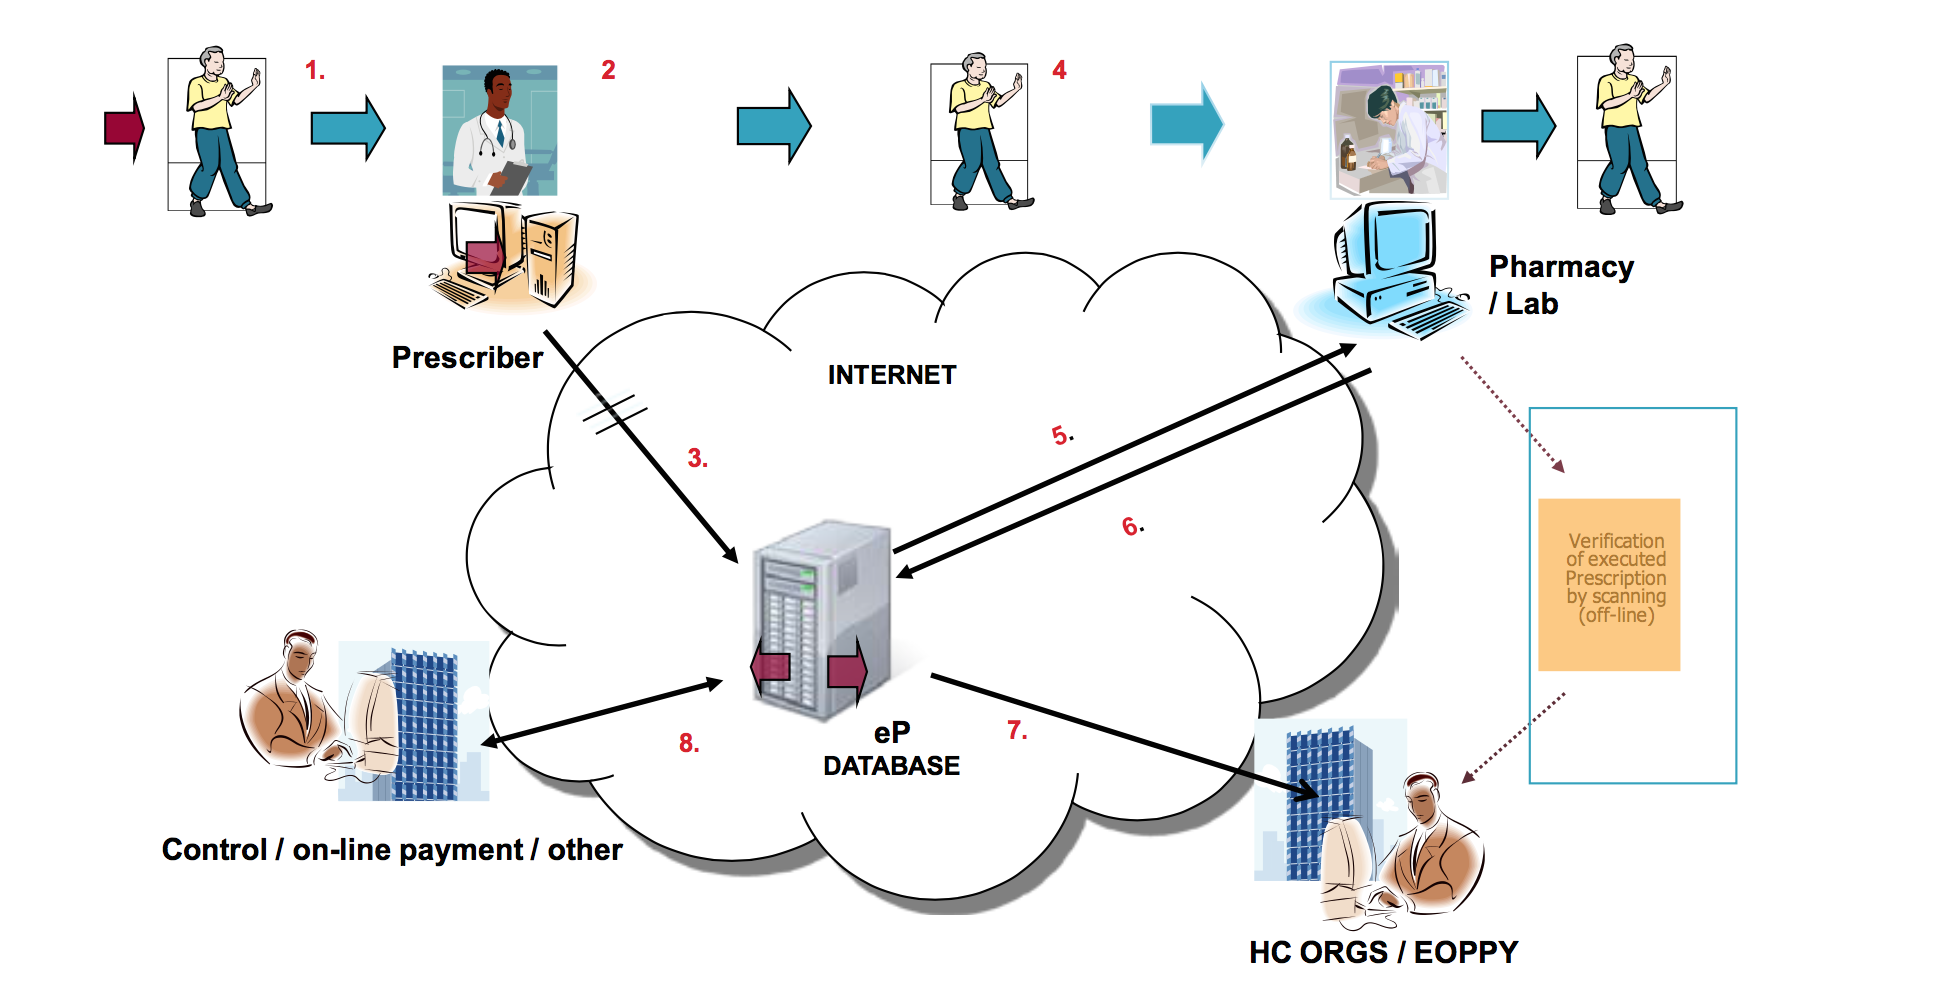
\includegraphics[width=0.7\textwidth]{e-prescr.png}
	    \caption{Το σύστημα E-prescription στην Ελλάδα. }
	    \label{fig:prescr}
	\end{figure}


	

	
	\subsection{Ηλεκτρονικός Ιατρικός Φάκελος (EMR)}
	

		Στην σύστημα υγείας η πληρότητα και η διαθεσιμότητα των δεδομένων και της πληροφορίας είναι ζωτικής σημασίας. Ημιτελείς πληροφορίες μπορούν να έχουν ως αποτέλεσμα κακή διάγνωση και θεραπεία, σπατάλη χρημάτων και πόρων ακόμα και να επιφέρουν καταστάσεις οι οποίες να απειλούν τη ζωή. Ο όγκος των πληροφοριών που σχετίζονται με την φροντίδα του ασθενούς έχει πολλαπλασιαστεί τα τελευταία χρόνια, γεγονός που οφείλεται σε μεγάλο ποσοστό στην ενσωμάτωση αυξημένου αριθμού εργαστηριακών και παρακλινικών εξετάσεων στους φακέλους των ασθενών.
	
		Ο ηλεκτρονικός ιατρικός φακέλου είναι ένα σύστημα σχεδιασμένο ώστε να υποστηρίζει την απόλυτη διαθεσιμότητα και την ακρίβεια ιατρικών ή άλλων πληροφοριών με σκοπό την παροχή ιατρικής περίθαλψης. Ο ηλεκτρονικός ιατρικός φάκελος ασθενούς είναι μία διαρκώς εξελισσόμενη έννοια και καθορίζεται ως μια συλλογή από ιατρικές πληροφορίες ιδιωτών ή πληθυσμών. Είναι αποθηκευμένος σε ψηφιακή μορφή, έχει την ικανότητα να διαμοιράζεται μεταξύ διαφορετικών ιατρικών λογισμικών και μπορεί να μεταφερθεί μέσω του δικτύου. Ένας ηλεκτρονικός φάκελος μπορεί να περιλαμβάνει μεγάλο πλήθος δεδομένων σε πλήρη ή περιληπτική μορφή, όπως δημογραφικά στοιχεία, ιατρικό ιστορικό φαρμακευτική αγωγή και αλλεργίες, προσωπικά στοιχεία όπως βάρος, ύψος, φύλο και άλλα.
		
		Σε αυτό το σημείο θα πρέπει να κάνουμε τον διαχωρισμό του ηλεκτρονικού ιατρικού φακέλου(EMR) και του ηλεκτρονικού φακέλου υγείας(EHR). O ηλεκτρονικός φάκελος υγείας (EHR) είναι μια εξελισσόμενη έννοια 
που αποθηκεύει ψηφιακά ένα υποσύνολο δεδομένων ή όλα τα δεδομένα σχετικά με τις ιατρικές πράξεις που έγιναν κατά τη διάρκεια της ζωής ενός ατόμου με σκοπό την υποστήριξη της ποιοτικής, προσβάσιμης και αποτελεσματικής συνέχειας στην παροχή υπηρεσιών υγείας. Ο ηλεκτρονικός ιατρικός φάκελος σε αντίθεση ορίζεται ως το αρχείο του ασθενούς που δημιουργήθηκε από τους παρόχους για συγκεκριμένες επισκέψεις του ασθενή σε νοσοκομεία και περιπατητική περιβάλλοντα, και η οποία μπορεί να χρησιμεύσει ως πηγή δεδομένων για τον ηλεκτρονικό φάκελο υγείας (EHR). Ο ηλεκτρονικός φάκελος υγείας (EHR) δημιουργείται και διατηρείται εντός ενός θεσμικού οργάνου, όπως ένα νοσοκομείο, ένα ολοκληρωμένο δίκτυο διανομής,μία κλινική, ή ένα γραφείο ιατρού για να δώσει σε όλους τους εμπλεκόμενους στην ιατρική φροντίδα πρόσβαση ιατρικό ιστορικό του ασθενούς.
	
	
		Ο κλασσικός ηλεκτρονικός ιατρικός φάκελος πρέπει κάθε χρονική στιγμή να περιέχει τουλάχιστον την επίσκεψη-επαφή του ασθενούς, το ιατρικό ιστορικό, τη διάγνωση, τη νοσηλεία (συνταγογράφηση, αποτελέσματα εργαστηριακών εξετάσεων ), τα δημογραφικά στοιχεία του ασθενούς (Όνομα, ΑΜΚΑ, Ασφαλιστικός φορέας, ομάδα αίματος κ.τ.λ.).


Το λογισμικό του ηλεκτρονικού φακέλου υγείας ουσιαστικά είναι ένα σύστημα διαχείρισης ιατρικών φακέλων που βασίζεται σε ηλεκτρονικούς υπολογιστές. Το γεγονός αυτό έχει ως αποτέλεσμα να αποθηκεύονται και να ανακτώνται δεδομένα γρήγορα και με ασφάλεια. Επιπλέον, τα δεδομένα επεξεργάζονται εύκολα και γρήγορα και μπορούν να μεταφερθούν σε οποιαδήποτε σύστημα, σε οποιαδήποτε απόσταση. Το σύστημα καταγραφής των δεδομένων γίνεται πιο αποτελεσματικό και περισσότερο πλήρες. Ο ηλεκτρονικός ιατρικός φάκελος εμπεριέχει μία πληθώρα δεδομένων, τα οποία έχουν διαφορετική μορφή. Το ιστορικό, η κλινική εξέταση και τα αποτελέσματα εργαστηριακών εξετάσεων, είναι σε μορφή κειμένου, οι εξετάσεις του ασθενούς (ακτινογραφίες, τομογραφίες - αξονικές, μαγνητικές, απλές - υπέρηχοι κ.α.) είναι σε μορφή στατικών εικόνων, τα ηλεκτροκαρδιογραφήματα είναι σε μορφή βιοσημάτων ,τα αποτελέσματα των ενδοσκοπικών εξετάσεων (γαστροσκόπηση κ.α. ) είναι σε μορφή βίντεο κ.λ.π.  Στον ηλεκτρονικό ιατρικό φάκελο , όλα τα δεδομένα ενσωματώνονται στον φάκελο του ασθενούς χωρίς να παίζει σημαντικό ρόλο η μορφή τους. Σε διάφορα σημεία του κειμένου του ιστορικού και της κλινικής εξετάσεως ενσωματώνονται ακτινολογικές ή βιοχημικές εξετάσεις, πράγμα που κάνει αμέσως εμφανή την συσχέτιση των εν λόγω εξετάσεων με την γενικότερη κατάσταση του ασθενούς.

Μερικά από τα πιο ουσιαστικά πλεονεκτήματα της χρήσης ενός συστήματος ηλεκτρονικού ιατρικού φακέλου είναι τα εξής
\begin{itemize}

\item Κέρδος χρόνου κατά την αναζήτηση και την συμπλήρωση στοιχείων του ιατρικού φακέλου. Η διείσδυση των τεχνολογιών αιχμής στον ιατρικό κόσμο εκσυγχρονίζεις την διαδικασία και κρατώντας όλα τα στοιχεία συγκεντρωμένα και με δυνατότητα άμεσης πρόσβασης - αναζήτησης επιταχύνουμε πολύ τις διαδικασίες.


\item

\item


\end{itemize}



Η ασφάλεια των ιατρικών δεδομένων είναι ένα σημαντικότατο θέμα για το οποίο, η
τεχνολογία μέσω του ηλεκτρονικού ιατρικού φακέλου έχει δώσει ουσιαστικές λύσεις, οι οποίες
μάλιστα μπορεί να θεωρηθούν αποτελεσματικότερες από αυτές που μέχρι σήμερα εφαρμόζονται
για την τήρηση και φύλαξη των ιατρικών φακέλων των ασθενών.
Στον ηλεκτρονικό ιατρικό φάκελο δίνεται ιδιαίτερη έμφαση στην προστασία των
προσωπικών δεδομένων τα οποία αρχειοθετούνται. Φυσικά λόγω της ευαισθησίας των
προσωπικών στοιχείων, πληρούνται όλες εκείνες οι προυποθέσεις ασφαλείας που εξασφαλίζουν
το αδιάβλητο των δεδομένων. 


	
	
	\subsection{epSOS}
	
		Η ανάγκη διασύνδεσης των συστημάτων υγείας και των πολιτικών που ακολουθούνται σε κάθε κράτος σχετικά με την υγεία στην Ευρωπαϊκή Ένωση, γίνεται όλο και πιο πιεστική, λόγω της αυξημένης κινητικότητας των ασθενών και των επαγγελματιών του ιατρικού τομέα και της διάδοσης των νέων ιατρικών τεχνολογιών και τεχνικών που αφορούν την τεχνολογία της πληροφορίας. Η διασύνδεση των διάφορων συστημάτων υγείας είναι απαραίτητη για την καλύτερη ποιότητα αλλά και την άμεση πρόσβαση των πολιτών στη διασυνοριακή περίθαλψη.  Πολλά κράτη μέλη της Ευρωπαϊκής Ένωσης έχουν αναπτύξει ηλεκτρονικά συστήματα σχετικά με τα αρχεία των ασθενών. Ο ηλεκτρονικός ιατρικός φάκελος του ασθενούς και η ηλεκτρονική συνταγογράφηση είναι δύο πολύ σημαντικά συστήματα τα οποία προάγουν την ασφαλή και αξιόπιστη ιατροφαρμακευτική περίθαλψη.	 	
	 	
	 	Η Ευρωπαϊκή Ένωση στα πλαίσια του στόχου της επικοινωνίας και της συνεργασίας των χωρών που εντάσσονται σε αυτή και την ύπαρξη κοινών οδηγιών στον τομέα της υγείας, τον Ιούλιο του 2008 σε συνεργασία με τους δημόσιους φορείς που έχουν αρμοδιότητα τις ηλεκτρονικές υπηρεσίες υγείας (ηλεκτρονικός ιατρικός φάκελος, ηλεκτρονικής συνταγογράφησης) ξεκίνησε ένα σημαντικό έργο, τον ευρωπαϊκό πιλότο epSOS (Έξυπνες Ανοιχτές Ηλεκτρονικές Υπηρεσίες για τους Ευρωπαίους Ασθενείς). Ο κύριος στόχος του epSOS είναι η ανάπτυξη ενός πρακτικού πλαισίου ηλεκτρονικής υγείας και κατάλληλων  υποδομών  στον τομέα της  Πληροφορικής και των Επικοινωνιών που θα επιτρέπουν την ασφαλή πρόσβαση των διάφορων μη εθνικών ευρωπαϊκών συστημάτων υγειονομικής περίθαλψης στις πληροφορίες αναφορικά με την υγεία του ασθενούς. Το epSOS είναι ένα έργο για την προώθηση της διαλειτουργικότητας της ηλεκτρονικής υγείας , το οποίο χρηματοδοτεί η Ευρωπαϊκή Ένωση και θέλει να χτίσει μια υποδομή υπηρεσιών, που θα επιτρέπει  τη διασυνοριακή διαλειτουργικότητα των συστημάτων ηλεκτρονικών μητρώων υγείας στην Ευρώπη, χωρίς να καταπατά όμως νομοθετικές ρυθμίσεις ή να υπερβαίνει τα ήδη υπάρχουσα εθνικά συστήματα. \cite{Dogac2012}


		Το epSOS αποτελείται από δύο χωριστές υπηρεσίες ηλεκτρονικής υγείας, τον ιατρικό φάκελο ασθενούς (patient medical record) και την ηλεκτρονική συνταγογράφηση (e-prescription),  για τις οποίες αναζητούνται διαλειτουργικές μέθοδοι στη διασυνοριακή επικοινωνία. Ειδικότερα, ο ιατρικός φάκελος ασθενούς  (patient medical record) στα πλαίσια του epSOS αποτελείται από στοιχεία τα οποία εμπεριέχουν γενικές πληροφορίες για τον ασθενή (π.χ. όνομα, ηλικία, γένος), σημαντικά κλινικά δεδομένα (π.χ. αλλεργίες, χρόνιες ασθένειες, χειρουργικές επεμβάσεις) , καθώς και τα τρέχοντα αλλά και παλαιότερα φαρμακευτικά σκευάσματα που λάμβανε. Ο φάκελος ασθενούς παρέχει τις βασικές πληροφορίες, οι οποίες βοηθούν τους επαγγελματίες του τομέα της υγείας να λάβουν σωστότερες και πιο ασφαλείς αποφάσεις σχετικά με την θεραπεία και τα φάρμακα που θα ακολουθήσουν οι ασθενείς. Οι πληροφορίες αυτές πρέπει να παρέχονται στην γλώσσα των εκάστοτε γιατρών, ώστε να μην προκύπτουν γλωσσικά εμπόδια. Η ηλεκτρονική συνταγογράφηση αφορά τη συνταγογράφηση των φαρμάκων με χρήση κατάλληλου λογισμικού και την ηλεκτρονική διαβίβασή τους. Στην ηλεκτρονική συνταγογράφηση η διαλειτουργικότητα μεταξύ των εθνικών συστημάτων είναι απαραίτητη όταν έχουμε έναν ασθενή ο οποίος χρειάζεται κάποιο φάρμακο, το οποίο έχει ήδη συνταγογραφηθεί σε κάποια άλλη χώρα.  Ο φαρμακοποιός θα πρέπει να αποκτήσει ηλεκτρονική πρόσβαση στη συνταγή, και όταν το φάρμακο αγοραστεί, το ηλεκτρονικό σύστημα θα πρέπει να ενημερώσει σχετικά με τα διανεμημένα φάρμακα το σύστημα υγειονομικής περίθαλψης της χώρας του ασθενούς. \cite{epSOS}
		
		 Το epSOS επιτυγχάνει την ασφαλή πρόσβαση των ασθενών σε πληροφορίες σχετικά με την υγεία τους για τα διάφορα ευρωπαϊκά συστήματα υγείας. Το σύστημα είναι φτιαγμένο για να εξυπηρετήσει έναν πολίτη της Ευρωπαϊκής Ένωσης  που ενώ είναι κατοικεί σε μια συγκεκριμένη χώρας δέχεται τακτικά υπηρεσίες υγείας σε μια άλλη χώρα εξαιτίας του καθώς εργάζεται σε αυτή τη χώρα ή βρίσκεται προσωρινά σε μία άλλη χώρα (π.χ. για τουρισμό ) και είναι ανάγκη να εκτελέσει μία ιατρική συνταγή της χώρας του ή χρειάζεται επείγουσα ιατρική περίθαλψη. Το epSOS παρέχει την κοινοτική οδηγία για τη διασυνοριακή ιατρική περίθαλψη, η οποία θα πρέπει να ενσωματωθεί στο εθνικό δίκαιο των κρατών μελών τα επόμενα χρόνια και επιπροσθέτως προτείνει τεχνικές λύσεις σε όλα τα επίπεδα διαλειτουργικότητας, όπως και σε θέματα πολιτικής και σε νομικά ζητήματα. επεκτείνεται πέρα από την έκδοση συστάσεων, μοντέλων οργάνωσης, και εργαλείων λογισμικού  στην  δοκιμή των αποτελέσματα αυτών μέσω πραγματικών πιλοτικών εφαρμογών σε πολλές ευρωπαϊκές περιφέρειες και χώρες.
		 


\section{Υλοποίηση}
\section{Δοκιμές}
